\documentclass[12pt,a4paper]{article}
\usepackage[utf8]{inputenc}
\usepackage[russian]{babel}
\usepackage[OT1]{fontenc}
\usepackage{amsmath}
\usepackage{amsfonts}
\usepackage{amssymb}
\usepackage{graphicx}
\graphicspath{{Images/}}
\usepackage[left=2cm,right=2cm,top=2cm,bottom=2cm]{geometry}
\usepackage{calc}
\usepackage{wrapfig}
\usepackage{setspace}
\usepackage{indentfirst}
\usepackage{subfigure}


\title{
Отчет о выполнении лабораторной работы 1.4.5

Изучение колебаний струны
}

\author{Мыздриков Иван Витальевич}
\date{\today}
\begin{document}

\maketitle
\newpage

\textbf{Цель работы:}исследовать зависимости частоты колебаний струны от величины натяжения, а также условий установления стоячей волны, получающейся в результате сложения волн, идущих в противоположных направлениях.

\textbf{В работе используются:} рейка со струной, звуковой генератор, постоянный магнит, разновесы.

\section{Теоретический материал}
Основное свойство струны -- гибкость, является следствием ее большой длины по сравнению с поперечными размерами. Даже струны, изготовленные из жестких материалов, практически не сопротивляются изгибанию, если размер изгибаемого участка значительно больше поперечного размера струны. Данный факт позволяет не учитывать при дальнейшей работе изгибные напряжения.

Горизонтально закрепленная струна провисает под действием поля тяжести, при отсутствии натяжения. Достаточно натянутую струну можно считать прямой, если ее концы закреплены на одном горизонтальном уровне. Учитывая этот факт, в дальнейшем действие силы тяжести учитываться не будет.

Натянутая струна с жестко закрепленными концами удобна для изучения колебаний. Это связанно с тем, что в струне можно непосредственно наблюдать простейшие типы колебаний и волн, измерять их параметры и сравнивать результаты наблюдения с результатами теоретических расчетов.

Движение элементов струны может быть вызвано изменением ее формы или передачей ей импульса. Натяжение струны стремиться вернуть ее в изначальное прямолинейное положение, и это приводит к тому, что возникает движение элементов струны. Возмущения бегут вдоль струны.

Скорость распространения подобного возмущения можно вычислить по формуле \ref{eq:velocity_of_deformation}.

\begin{equation}
	u = \sqrt{\frac{F}{\rho_{l}}},
	\label{eq:velocity_of_deformation}
\end{equation}
где $F -- $ сила натяжения струны, $\rho_{l} -- $ масса струны на единицу длины.

При заданной частоте $\nu$ длина волны определяется по формуле:

\begin{equation}
	\lambda = \frac{u}{\nu}
\end{equation}

Частоты собственных колебаний струны определяются формулой:

\begin{equation}
	\nu_{n} = n\frac{u}{2l},
	\label{eq:frequency_velocity_equation}
\end{equation}

где $n -- $ число полуволн, $l -- $ длина струны.

\section{Выполнение работы}

Перед началом выполнения работы опишем грузы, используемые в работе для нагружения струны и изменения ее натяжения. Масса грузов и их номер занесены в таблицу \ref{tab:mass_of_load}. Полная масса нагрузки для отдельного измерения приведена в таблице \ref{tab:mass_of_load_for_all_measuring}

\begin{table}[h!]
\centering
\begin{tabular}{|c|c|c|c|c|c|c|}
\hline
№ груза     & 1   & 2     & 3     & 4     & 5  & подвес  \\ \hline
Масса груза $M,$ г & - & 482.4 & 493.2 & 339.2 & 493.9 & 1016 \\ \hline
\end{tabular}
\caption{Масса грузов, используемых в ходе выполнения работы}
\label{tab:mass_of_load}
\end{table}

Величина нагрузки и массы грузов связаны следующим образом:

\begin{equation}
	T_{i} = \left(m_{\text{подвеса}} + M_{2} + \sum_{k=2}^i M_{k}\right)g
\end{equation}

\begin{table}[h!]
\centering
\begin{tabular}{|c|c|c|c|c|c|}
\hline
№ измерения        & 1      & 2      & 3      & 4      & 5           \\ \hline
Полная нагрузка $T$, Н & 10,16 & 14.9 &	19.9 &	23.3 &	28.2 
 \\ \hline
\end{tabular}
\caption{Полная масса нагрузки для каждого измерения.}
\label{tab:mass_of_load_for_all_measuring}
\end{table}

Результаты измерения частот гармоник для каждого значения нагрузки занесены в таблицу \ref{tab:measuring_results}.

Формула, описывающая зависимость скорости u от нагрузки, приложенной к струне имеет вид \ref{eq:velocity_force_equation}:

\begin{equation}
	\nu_{n} = \frac{n}{2l} \sqrt{\frac{F}{\rho_{l}}}
	\label{eq:velocity_force_equation}
\end{equation}

По результатам измерений, занесенным в таблицу \ref{tab:measuring_results}, построим графики зависимости частоты $\nu_{n}$ от номера гармоники $n$. График изображен на рисунке \ref{fig:grapfic_frequency_force_depend}. С помощью МНК определим значение коэффициента угла наклона для данного графика. Из формулы \ref{eq:frequency_velocity_equation} видно, что данный коэффициент равен $\frac{u}{2l}$, значит, из данных зависимостей определим значение скорости $u$

\begin{table}[h!]
\centering
\begin{tabular}{|c|c|c|c|c|c|}
\hline
№ измерения        & 1        & 2        & 3        & 4        & 5        \\ \hline
$\nu_{1}$, Гц      & 136.2    & 162.2    & 187      & 202.5    & 220.7    \\ \hline
$\nu_{2}$, Гц      & 272.4    & -        & -        & -        & -        \\ \hline
$\nu_{3}$, Гц      & 187      & 486.6    & 561      & 607.2    & 662.1    \\ \hline
$\nu_{4}$, Гц      & 408.6    & -        & -        & -        & -        \\ \hline
$\nu_{5}$, Гц      & 544.8    & 811      & 935      & 1012.2   & 1103.5   \\ \hline
$\nu_{6}$, Гц      & 681      & -        & -        & -        & - 		  \\ \hline
$\nu_{7}$, Гц      & 817.2    & 1135.4   & 1309     & 1417     & 1544.9   \\ \hline
$\nu_{8}$, Гц      & 953.4    & -        & -        & -        & -        \\ \hline
$\nu_{9}$, Гц      & (нет видимых колебаний)        & -        & -        & -        & -        \\ \hline
\end{tabular}

\caption{Результаты измерений частот гармоник в зависимости от массы нагрузки.}
\label{tab:measuring_results}
\end{table}

\begin{figure}[h!]
	\begin{center}
		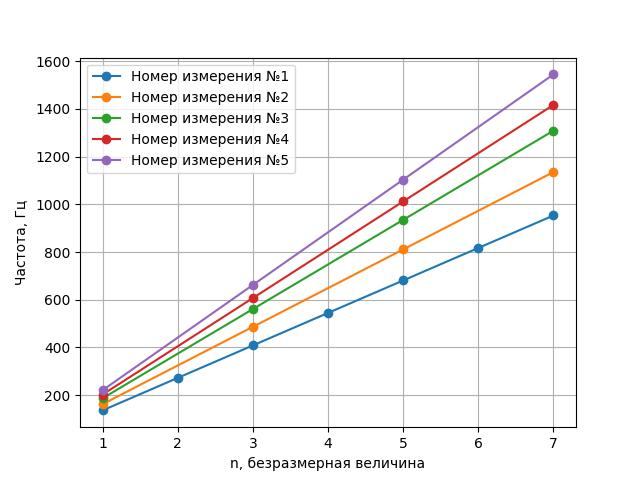
\includegraphics[width = 0.85\textwidth]{res1}
		\caption{Графики зависимости частоты гармоники от нагрузки для различных n}
		\label{fig:grapfic_frequency_force_depend}
	\end{center}
\end{figure}

Определим значения скорости u для каждого значения нагрузки. Значения занесем в таблицу \ref{tab:velocity_with_mistakes}

\begin{table}[h]
\centering
\begin{tabular}{|c|c|c|c|c|c|}
\hline
$\overline{u}$  & 133.7 & 162.4 & 187.2 & 202.5 & 222.9 \\ \hline
$\varepsilon_{u}$   & 0,01 & 0,013 & 0,015 & 0,016 & 0,017  \\ \hline
$\sigma_{u}$     & 1.3   & 2.1   & 2.8   & 3.4   & 3.9  \\ \hline

\end{tabular}
\caption{Определение погрешности измерения скорости}
\label{tab:velocity_with_mistakes}
\end{table}

Используя данные таблицы \ref{tab:velocity_with_mistakes}, построим график зависимости $u^{2}\left(F\right)$. Данный график изображен на рисунке \ref{fig:u_sqr_depends_of_force}.

\begin{figure}[h!]
	\begin{center}
		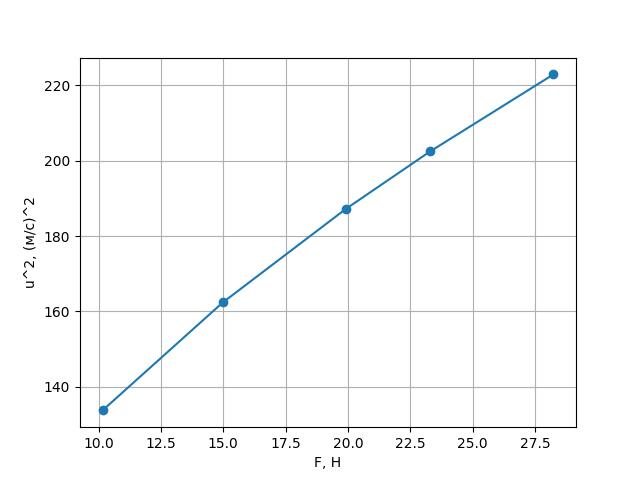
\includegraphics[width = 0.8\textwidth]{res2}
		\caption{Зависимость $u^{2}\left(F\right)$}
		\label{fig:u_sqr_depends_of_force}
	\end{center}
\end{figure}

C помощью МНК определим значение коэффициента угла наклона данного графика:

$ k = 1759 \pm 25$

Определим, как связан угловой коэффициент и величина линейной плотности струны:

$k = \frac{1}{\rho_{l}}$

Из данных соотношений получаем значение $\rho_{l} = 568.5 \pm 8 \frac{\text{мг}}{\text{м}}$. Значение, указанное на данной установке -- $568,4 \pm 0,1$  $\frac{\text{мг}}{\text{м}}$(Отклонение составляет $0,1 \approx 0,1 \%$)



Значит, определенное таким образом значение линейной плотности струны совпадает с истинной линейной плотностью струны в пределах погрешности.
\begin{figure}[h!]
	\begin{center}
		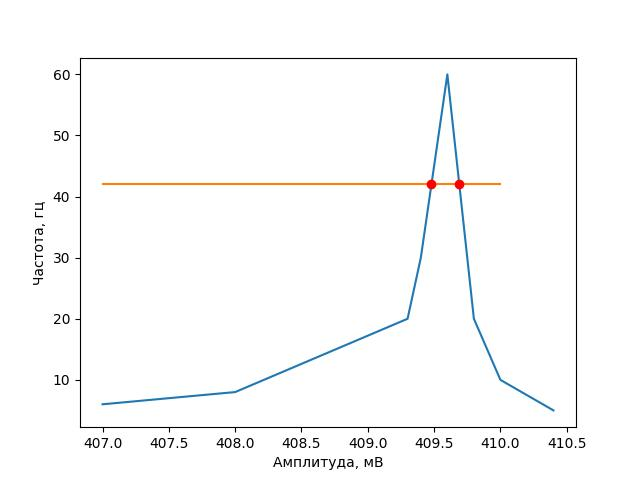
\includegraphics[width = 0.8\textwidth]{res3}
		\caption{Зависимость амплитуды от частоты}
		\label{fig:u_sqr_depends_of_force}
	\end{center}
\end{figure}

\newpage
Для определения добротности найдем несколько точек с разными амплитудами в близи резонансной частоты.
После найдем точки, где амплитуда будет в 70\% от максимальной амплитуды и по формуле вычислим добротность:

\begin{equation}
	\text{Q} = \frac{\nu_{\text{рез}}}{\Delta\nu},
	\label{eq:frequency_velocity_equation}
\end{equation}

Полученное значение $Q = 1905 \pm 55$
\section{Результаты}

\begin{enumerate}
	\item Во время выполнения работы было подтверждено несколько теоретических зависимостей между физическими величинами. С точностью $\varepsilon_{\nu_{1}} = 0,022$ подтверждена формула для определения частот гармоники струны. С точностью  $\overline{\varepsilon_{u}} = 0,03$ подтверждена формула для определения скорости распространения волны в твердом теле под действием внешней силы.
	\item Полученные графики имеют вид, предсказанный теоретически. Относительно большое значение относительной погрешности определения частоты 11 гармоники для массы нагрузки, соответствующей 3 грузам, объясняется ошибочным измерением частоты данной гармоники, что видно из графика. 
	
	% $\rho_{l} = 573 \pm 8 \frac{\text{мг}}{\text{м}}$
	
	% $\rho_{\text{уст}} = 568,4 \pm 0,1 \frac{\text{мг}}{\text{м}}$

\end{enumerate}
\end{document}